\documentclass{scrartcl}
\usepackage{listings}
\usepackage{xcolor}
\definecolor{lightcyan}{HTML}{E0FFFF}
\usepackage[colorlinks=true, urlcolor=blue, linkcolor=red]{hyperref}
\usepackage{graphicx}


\begin{document}
    \lstset{
        language=Java,
        numbers=left,
        stepnumber=1,
        numbersep=5pt,
        backgroundcolor=\color{lightcyan},
        showspaces=false,
        showstringspaces=false,
        showtabs=false,
        tabsize=2,
        captionpos=b,
        breaklines=true,
        breakatwhitespace=true,
        title=\lstname,
    }

\section{Sources}

\begin{itemize}
    \item \url{https://redips789.github.io/spring-certification/Spring-Certification.html}
    \item \url{https://www.baeldung.com/inversion-control-and-dependency-injection-in-spring}
    \item \url{https://www.baeldung.com/inversion-control-and-dependency-injection-in-spring}


    \item \url{https://www.baeldung.com/spring-bean-names}
    \item \url{https://www.baeldung.com/spring-core-annotations}
    \item \url{https://www.baeldung.com/spring-bean-annotations}
    \item \url{https://www.baeldung.com/spring-component-scanning}
    \item \url{https://www.baeldung.com/spring-annotations-resource-inject-autowire}
    \item \url{https://www.digitalocean.com/community/tutorials/spring-bean-life-cycle}
\end{itemize}

\section{Bean Lifecycle}
\subsection{Overview}

From a bird's eye, everything that happens before a bean is ready to use can be assigned to one of three phases (see fig. \ref{fig:bean-lifecycle-3}):

\begin{itemize}
    \item Loading and maybe modifying bean definitions
    \item Instantiating beans
    \item Initializing beans
\end{itemize}

\begin{figure}
    \centering
    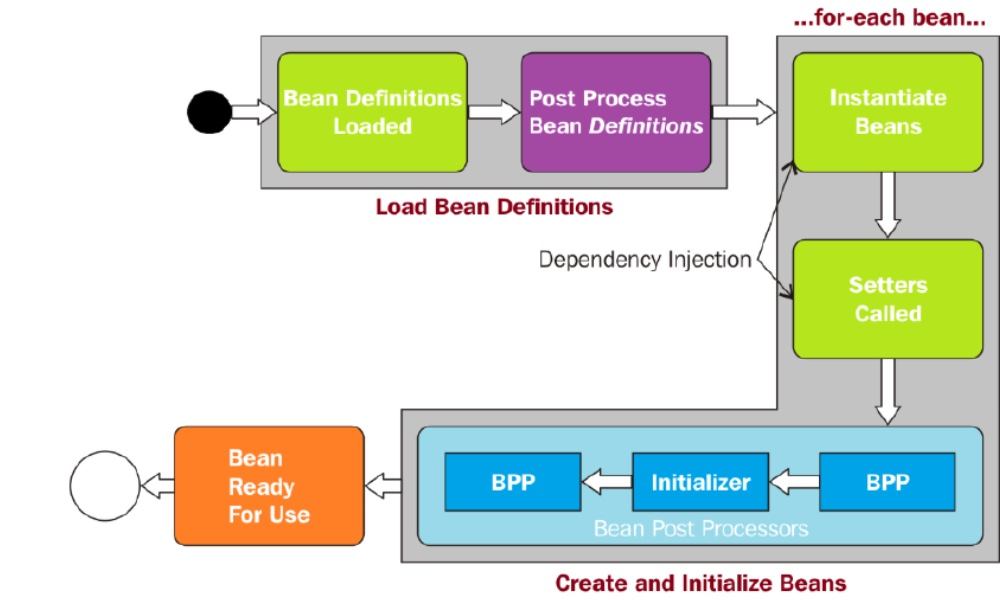
\includegraphics[width=1\linewidth]{bean-lifecycle-3}
    \caption{Lifecycle overview}
    \label{fig:bean-lifecycle-3}
\end{figure}

Figure \ref{fig:bean-lifecycle-2} focuses on pre-initialization.

\begin{figure}
    \centering
    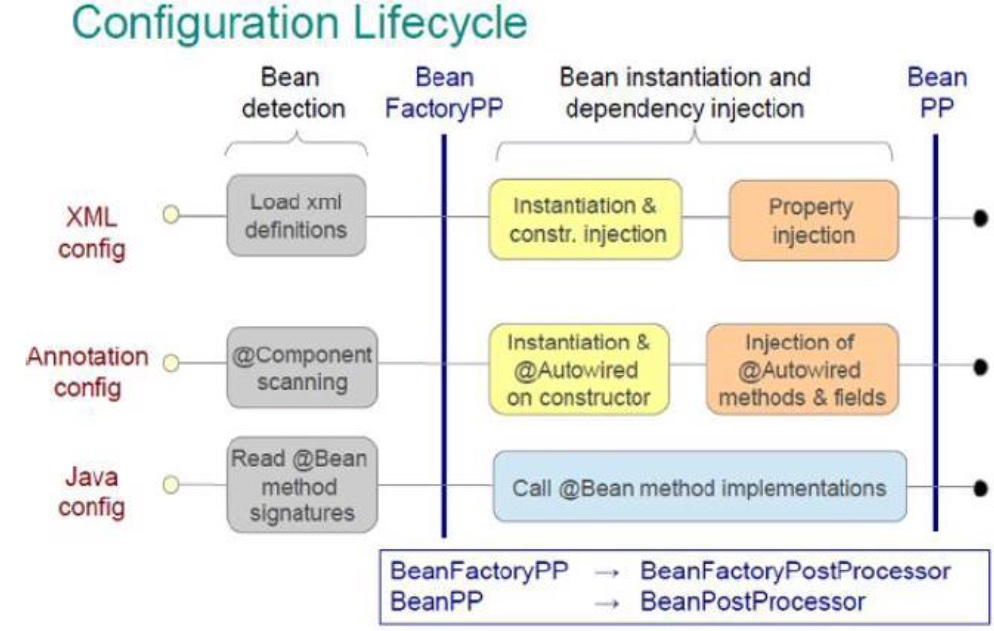
\includegraphics[width=1\linewidth]{bean-lifecycle-2}
    \caption{Zooming in on pre-instantiation}
    \label{fig:bean-lifecycle-2}
\end{figure}

On the other hand, fig. \ref{fig:bean-lifecycle-1} zooms in on post-instantiation.

\begin{figure}
    \centering
    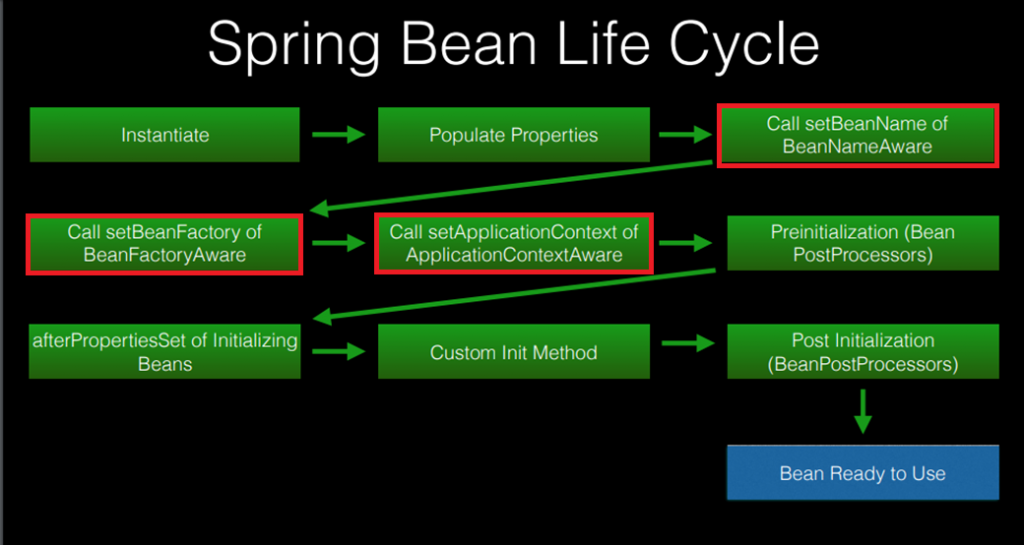
\includegraphics[width=1\linewidth]{bean-lifecycle-1}
    \caption{Zooming in on post-instantiation}
    \label{fig:bean-lifecycle-1}
\end{figure}


See https://www.digitalocean.com/community/tutorials/spring-bean-life-cycle for code to display the order of invocations.

\subsubsection{Load bean definitions, creating an ordered graph}
In this step, all the configuration files – @Configuration classes or XML files – are processed. For annotation-based configuration, all the classes annotated with @Components are scanned to load the bean definitions.

Bean definitions are passed to a BeanFactory, each under its id and type. For example, ApplicationContext is a BeanFactory.

Then, BeanFactoryPostProcessors are run.

\subsubsection{Instantiate and run BeanFactoryPostProcessors}
In a Spring application, a BeanFactoryPostProcessor can modify the definition of any bean.
The BeanFactory object is passed as an argument to the postProcess() method of the BeanFactoryPostProcessor. BeanFactoryPostProcessor then works on the bean definitions or the configuration metadata of the bean before the beans are actually created.
Spring provides several useful implementations of BeanFactoryPostProcessor, such as reading properties and registering a custom scope. We can write your own implementation of the BeanFactoryPostProcessor interface. To influence the order in which bean factory post processors are invoked, their bean definition methods may be annotated with the @Order annotation. If you are implementing your own bean factory post processor, the implementation class can also implement the Ordered interface.

\begin{figure}
    \centering
    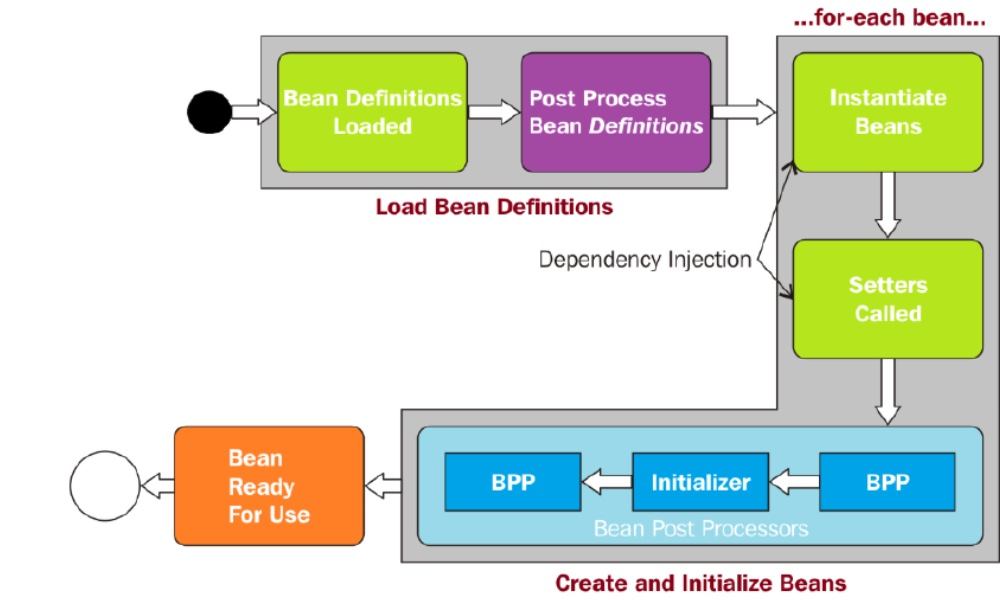
\includegraphics[width=1\linewidth]{bean-lifecycle-3}
    \caption{}
    \label{fig:bean-lifecycle-1}
\end{figure}

\subsubsection{Instantiate beans}
Injects values and bean references into beans’ properties.

\subsubsection{Call BeanNameAware’s setBeanName() for each bean implementing it}

\subsubsection{Call BeanFactoryAware’s setBeanFactory() passing the bean factory for each bean implementing it}

\subsubsection{Call ApplicationContextAware’s setApplicationContext for each bean implementing it}

\subsubsection{Before initialization: Run pre-initialization BeanPostProcessors}
The Application context calls postProcessBeforeInitialization() for each bean implementing BeanPostProcessor.

\begin{lstlisting}
   public interface BeanPostProcessor {

       /**
       * Apply this {@code BeanPostProcessor} to the given new bean instance before any bean's initialization callbacks (like InitializingBean's afterPropertiesSet
       * or a custom init-method).
       **/
       @Nullable
       default Object postProcessBeforeInitialization(Object bean, String beanName) throws BeansException {
           return bean;
       }

       /**
       * Apply this {@code BeanPostProcessor} to the given new bean instance after any bean initialization callbacks (like InitializingBean's afterPropertiesSet
       * or a custom init-method).
       */
       @Nullable
       default Object postProcessAfterInitialization(Object bean, String beanName) throws BeansException {
           return bean;
       }
   }
\end{lstlisting}

In postProcessBeforeInitialization and postProcessAfterInitialization, a bean implementing BeanPostProcessor can return anything it wants - even something completely different!

Figure \ref{fig:custom_bean_postprocessor} shows a no-op implementation.

\begin{figure}
    \centering
    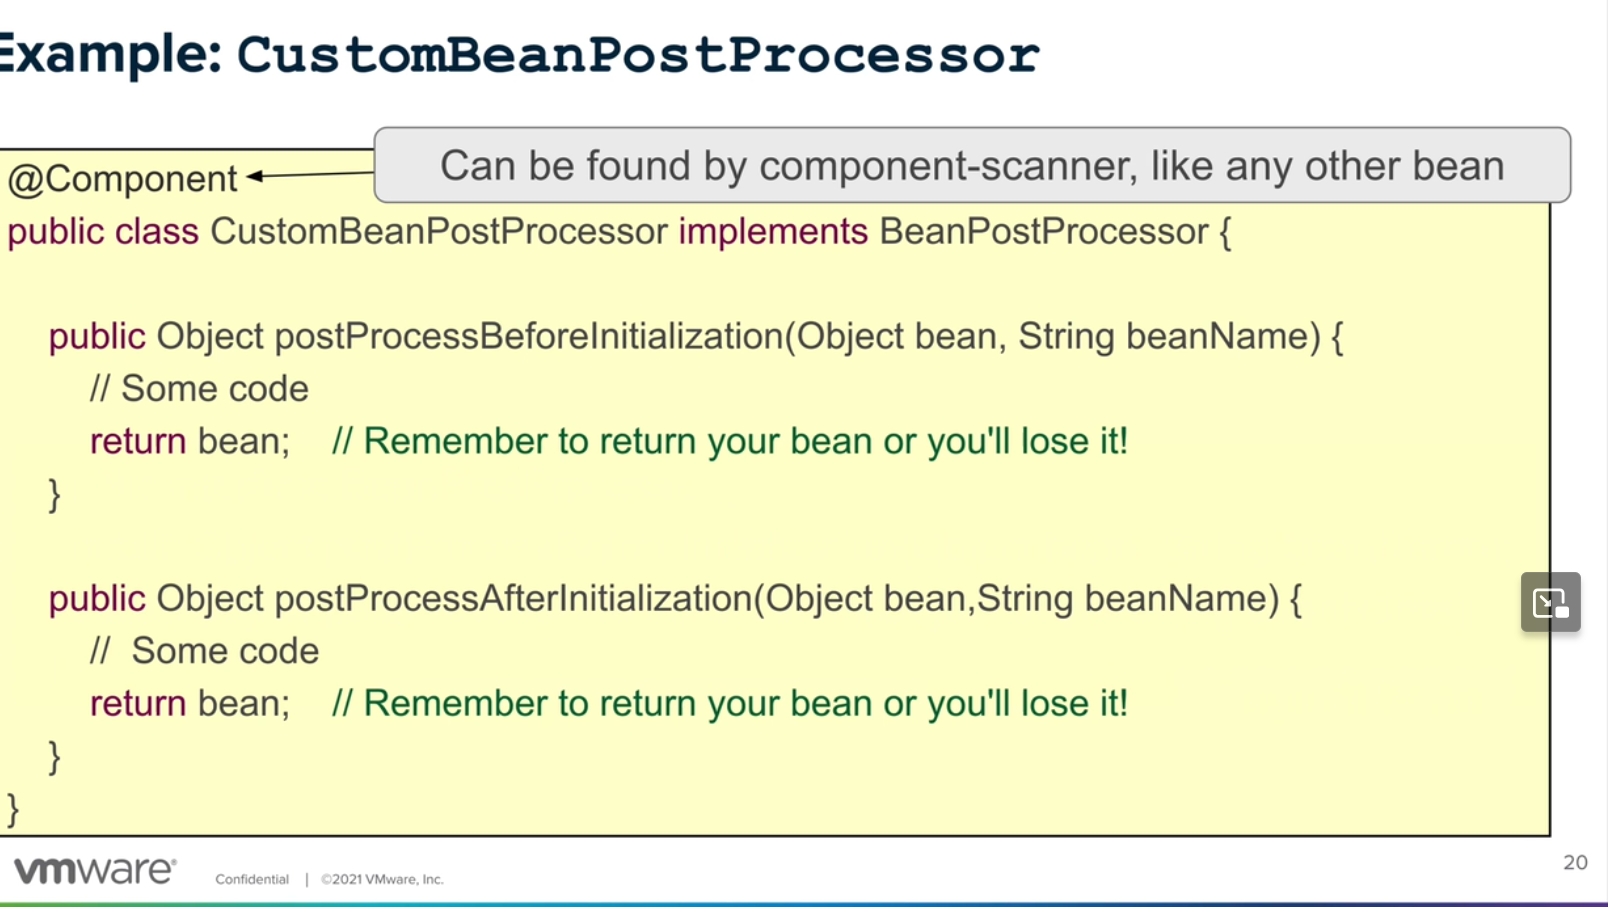
\includegraphics[width=1\linewidth]{custom_bean_postprocessor}
    \caption{Custom bean postprocessor}
    \label{fig:custom_bean_postprocessor}
\end{figure}

\subsubsection{Initialization: Call InitializingBean’s afterPropertiesSet()}
If a bean implements the InitializingBean interface, Spring calls its afterPropertiesSet() method. Used to initialize processes,  load resources, etc. This approach is simple to use but it’s not recommended because it will create tight coupling with the Spring framework in our bean implementations.

\begin{lstlisting}
public interface InitializingBean {

    /**
    * Invoked by the containing BeanFactory after it has set all bean properties.
    * This method allows the bean instance to perform validation of its overall configuration and final initialization when all bean properties have been set.
    */
    void afterPropertiesSet() throws Exception;

}
\end{lstlisting}

\subsubsection{Initialization: Init Method, @PostConstruct}
Instead of implementing InitializingBean, you can use the init-method of the bean tag, the initMethod attribute of the @Bean annotation, and JSR 250's @PostConstruct  annotation.
Here we use the init-method attribute:

\begin{lstlisting}
    <bean name="myEmployeeService" class="com.journaldev.spring.service.MyEmployeeService"
    init-method="init" destroy-method="destroy">
    <property name="employee" ref="employee"></property>
    </bean>
\end{lstlisting}

Using init-method is a solution when you don't own the class (and so, can't annotate it).

And here, the @PostConstruct annotation.

\begin{lstlisting}
    @PostConstruct
    public void init(){
        System.out.println("MyService init method called");
    }
\end{lstlisting}

@PostConstruct and init-method are enabled by Spring's  CommonAnnotationBeanPostProcessor. This is a
BeanPostProcessor implementation that supports common Java annotations out of the box, in particular the JSR-250 annotations in the javax.annotation package.

It includes support for the javax.annotation.PostConstruct and javax.annotation.PreDestroy annotations - as init annotation and destroy annotation, respectively - through inheriting from InitDestroyAnnotationBeanPostProcessor with pre-configured annotation types.

\begin{lstlisting}
    public class CommonAnnotationBeanPostProcessor extends InitDestroyAnnotationBeanPostProcessor
    implements InstantiationAwareBeanPostProcessor, BeanFactoryAware, Serializable {...}

\end{lstlisting}

\subsubsection{After initialization: Run post-initialization BeanPostProcessors}
The application context calls postProcessAfterInitialization() for each bean implementing BeanPostProcessor.

\subsubsection{Bean ready to use}
Your beans remain live in the application context until it is closed by calling the close() method of the application context.

\subsubsection{Custom destruction}
If a bean implements the DisposableBean interface, Spring calls its destroy() method to destroy any process or clean up the resources of your application. There are other methods to achieve this step-for example, you can use the destroy-method of the tag, the destroyMethod attribute of the `@Bean` annotation, and JSR 250's `@PreDestroy` annotation.

\section{Dependency injection}
\subsection{Constructor-based}

    In the case of constructor-based dependency injection, the container will invoke a constructor with arguments each representing a dependency we want to set.
    This is the recommended way.

    \begin{lstlisting}
        @Configuration
        public class AppConfig {
            @Bean
            public Item item1() {
                return new ItemImpl1();
            }
            @Bean
            public Store store() {
                return new Store(item1());
            }
        }
    \end{lstlisting}

    Resp.

    \begin{lstlisting}
        <bean id="item1" class="org.baeldung.store.ItemImpl1" />
        <bean id="store" class="org.baeldung.store.Store">
        <constructor-arg type="ItemImpl1" index="0" name="item" ref="item1" />
        </bean>
    \end{lstlisting}

\subsection{Method-based}

    For setter-based DI, the container will call setter methods of our class after invoking a no-argument constructor or no-argument static factory method to instantiate the bean.

    \begin{lstlisting}
        @Bean
        public Store store() {
            Store store = new Store();
            store.setItem(item1());
            return store;
        }
    \end{lstlisting}

    Resp.

    \begin{lstlisting}
        <bean id="store" class="org.baeldung.store.Store">
        <property name="item" ref="item1" />
        </bean>
    \end{lstlisting}

\subsection{Field-based}

    In field-based DI, we can inject the dependencies by marking them with an @Autowired annotation. (This even works for private fields.)
    Field-based injection is not recommended - e.g., it makes testing harder.

    \begin{lstlisting}
        public class Store {
            @Autowired // deprecated
            private Item item;
        }
    \end{lstlisting}


\section{Configuration: Implicit vs. Explicit}

    Also referred to as Java-based (decoupled) and annotation-based.

    with both types, bean naming works differently - see \ref{sec:bean-naming}.

\subsection{Java-based}

    Takes place completely in @Configuration classes. E.g.,

    \begin{lstlisting}
        @Configuration
        public class MyConfig {
        @Bean
        public AccountRepo AccountRepo(){}
        }
    \end{lstlisting}

\subsection{Annotation-based}

    Bean definition and wiring take place completely in POJOs. For this to work, we need to enable component scanning.

    \begin{lstlisting}
        @Configuration
        @ComponentScan
        public class MyConfig {}

        @Component
       public class AccountRepo {}
    \end{lstlisting}


\subsection{Spring Boot Auto-Configuration}

    When @EnableAutoConfiguration is present, beans annotated with @AutoConfiguration  will be configured.

    In spring-boot-autoconfigure.jar, /META-INF/spring/org.springframework.boot.autoconfigure.AutoConfiguration.imports lists the classes by default autoconfigured by Spring.

    Spring's DataSourceAutoConfiguration class is one example. See fig. \ref{fig:datasourceautoconfiguration}.

    \begin{figure}
    \centering
    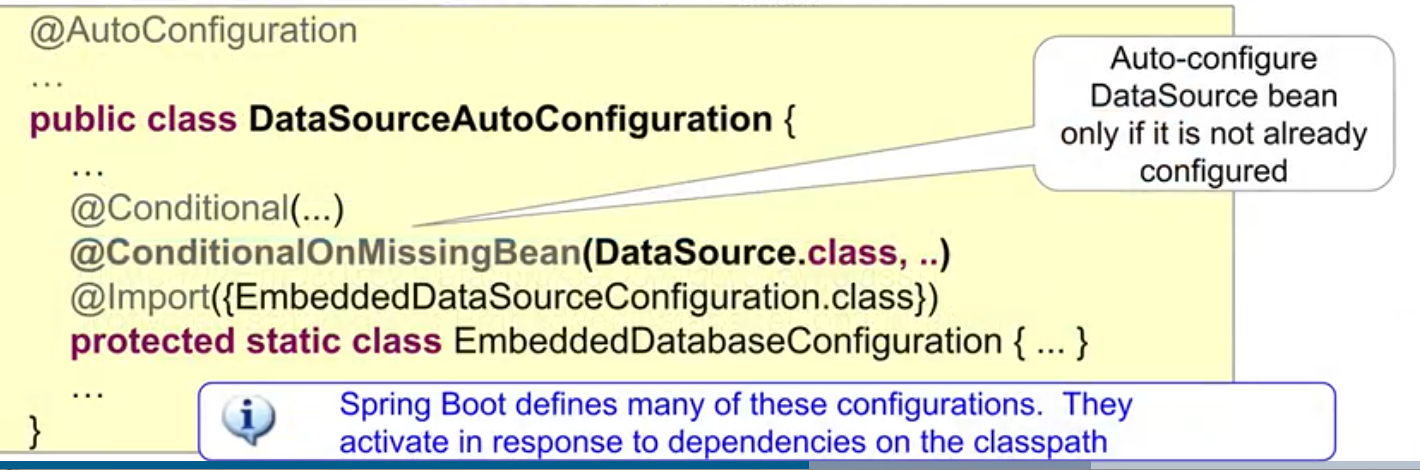
\includegraphics[width=1\linewidth]{datasourceautoconfiguration}
    \caption{Spring's DataSourceAutoConfiguration class.}
    \label{fig:datasourceautoconfiguration}
    \end{figure}


\section{Annotations}
\subsection{Annotations for dependency injection}
\subsubsection{@Autowired}
    @Autowired marks a dependency which Spring is going to resolve and inject. We can use this annotation with constructor, setter, or field injection. E.g.,

    \begin{lstlisting}
        class Car {
            @Autowired
            Engine engine;
        }
    \end{lstlisting}

    Starting with version 4.3, we don’t need to annotate constructors with @Autowired explicitly unless we declare at least two constructors.

    @Autowired matches by type. If there are several classes matching the required type (e.g., implementing the same interface), @Autowired needs to be supplemented by @Qualifier:

    \begin{lstlisting}
        @Component("Repo1")
        class Repo1 implements Repo {}

        @Component("Repo2")
        class Repo2 implements Repo {}

        @Component
        public class Service1 implements ServiceX {
            public Service1(@Qualifier("Repo2") Repo){}

        }

    \end{lstlisting}

    If there is no @Qualifier given, @Autowired looks for a matching bean name ( = bean id).
    Here, Spring will look for a bean named x:

    \begin{lstlisting}
        // constructor injection
        @Autowired
        public MyBean(X x){}

       // method injection
       @Autowired
       public setX(X x){}

       // field injection
       @Autowired
       private X x;
    \end{lstlisting}

\subsubsection{@Bean}

    @Bean marks a factory method which instantiates a Spring bean.

    \begin{lstlisting}
        @Bean
        Engine engine() {
            return new Engine();
        }
    \end{lstlisting}

    Spring calls these methods when a new instance of the return type is required. All methods annotated with @Bean must be in @Configuration classes.


\subsubsection{@Resource}

The @Resource annotation matches by name, type, or qualifier (in this order). It is applicable to setter and field injection.
Here’s an example injecting a field. Note that the bean id and the corresponding reference attribute value must match:

\begin{lstlisting}
    @Configuration
    public class MyAppContext {
        @Bean(name="namedFile")
        public File namedFile() {
            File namedFile = new File("namedFile.txt");
            return namedFile;
        }
    }

    @ContextConfiguration(
    loader=AnnotationConfigContextLoader.class,
    classes= MyAppContext.class)
    public class Xxx {
        @Resource(name="namedFile")
        private File defaultFile;
    }
\end{lstlisting}

\subsubsection{@Inject}

The @Inject annotation matches by type, qualifier, or name (in this order). It is applicable to setter and field injection. With @Inject, the class reference variable's name and the bean name don’t have to match.

To use the @Inject annotation, declare the javax.inject library as a Gradle or Maven dependency.

\begin{lstlisting}
    public class MyAppContext {
        @Bean
        // no bean name specified - method name is used
        public File getSomeFile() {
            File namedFile = new File("namedFile.txt");
            return namedFile;
        }
    }

    @ContextConfiguration(
    loader=AnnotationConfigContextLoader.class,
    classes= MyAppContext.class)
    public class Xxx {
        @Inject
        private File defaultFile;
    }
\end{lstlisting}

\subsubsection{@Value}

    We can use @Value for injecting property values into beans. It’s compatible with constructor, setter, and field injection. E.g.,

    \begin{lstlisting}
        Engine(@Value("8") int cylinderCount) {
            this.cylinderCount = cylinderCount;
        }
    \end{lstlisting}

    This is an alternative to making explicit use of Spring's Environment bean. E.g.

    \begin{lstlisting}
       public DataSource dataSource(
        @Value("${db.driver}") String driver,
        ...
        )
        }
    \end{lstlisting}

\subsubsection{@DependsOn}

    We can use this annotation to make Spring initialize other beans before the annotated one. Usually, this behavior is automatic, based on the explicit dependencies between beans. We only need this annotation when the dependencies are implicit, for example, JDBC driver loading or static variable initialization. E.g.,

     \begin{lstlisting}
        @Bean
        @DependsOn("fuel")
        Engine engine() {
            return new Engine();
        }
    \end{lstlisting}

\subsubsection{@Lazy}

    This annotation behaves differently depending on where exactly we place it.

    \begin{itemize}
        \item In an @Bean-annotated bean factory method, it is used to delay the method call (hence the bean creation)
        \item With an @Configuration class, all contained @Bean methods will be affected
        \item For all other @Component classes,  they will be initialized lazily when so annotated.
        \item @Autowired constructors, setters, and fields will be loaded lazily (via proxy).
    \end{itemize}

    \begin{lstlisting}
        @Configuration
        @Lazy
        class VehicleFactoryConfig {

            @Bean
            @Lazy(false)
            Engine engine() {
                return new Engine();
            }
        }
    \end{lstlisting}

\subsubsection{@Scope}

    @Scope is used to define the scope of a @Component class or a @Bean definition. It can be either singleton, prototype, request, session, globalSession or some cust@Component.

\subsection{Context Configuration Annotations}

\subsubsection{@Import}

    With @import, we can use specific @Configuration classes without component scanning.

    \begin{lstlisting}
        @Import(VehiclePartSupplier.class)
        class VehicleFactoryConfig {}
    \end{lstlisting}

\subsubsection{@ImportResource}

    We can import XML configurations with @ImportResource. We can specify the XML file locations with the locations argument, or with its alias, the value argument:

    \begin{lstlisting}
        @Configuration
        @ImportResource("classpath:/annotations.xml")
        class VehicleFactoryConfig {}
    \end{lstlisting}

\subsubsection{@PropertySource}

    With this annotation, we define property files for application settings.

    \begin{lstlisting}
        @Configuration
        @PropertySource("classpath:/annotations.properties")
        @PropertySource("classpath:/vehicle-factory.properties")
        class VehicleFactoryConfig {}
    \end{lstlisting}

    These properties can be used by Spring's Environment bean, in addition to environment variables and Java system properties.

    Allowed prefixes are classpath:, file:, and http:.

\subsection{Bean annotations}

\subsubsection{@Profile}

    Profiles are a way to group bean definitions, for example:

     \begin{itemize}
        \item dev, test, prod environment
        \item jdbc, jpa [implementations]
    \end{itemize}

   The @Profile annotation may be used in any of the following ways:

   \begin{itemize}
       \item At class level in @Configuration classes.
       \item At class level in classes annotated with @Component or annotated with any other annotation that in turn is annotated with @Component.
       \item On methods annotated with the @Bean annotation.
   \end{itemize}

    To define alternative beans with different profile conditions, use distinct Java method names pointing to the same bean name via the @Bean name attribute:

    \begin{lstlisting}
        @Bean("dataSource")
        @Profile("development")
        public DataSource standaloneDataSource(){

        @Bean("dataSource")
        @Profile("production")
        public DataSource jndiDataSource() throws Exception {}

    \end{lstlisting}

   Spring uses two separate properties when determining which profiles are active, spring.profiles.active and spring.profiles.default:

    \begin{itemize}
       \item If spring.profiles.active is set,  then its value determines which profiles are active.
       \item If spring.profiles.active isn’t set, then Spring looks to spring.profiles.default.
       \item If neither spring.profiles.active nor spring.profiles.default is set, only those beans that aren’t defined as being in a profile are created.
    \end{itemize}

   These properties can be set on the command line:

   \begin{lstlisting}[language=bash]
       -Dspring.profiles.active=embedded.jpa
   \end{lstlisting}

   , programmatically:

   \begin{lstlisting}
       System.setProperty("spring.profiles.active", "embedded.jpa");
   \end{lstlisting}

   , or via an annotation (@ActiveProfiles; integration tests only).


\subsubsection{@ComponentScan}

    The @ComponentScan annotation is used together with @Configuration.

    @ComponentScan can be used with and without arguments.

    Without arguments, @ComponentScan  tells Spring to scan the current package and all of its sub-packages.

    With arguments, @ComponentScan tells which packages or classes to scan. E.g., specifying packages:

    \begin{lstlisting}
        @Configuration
        @ComponentScan(basePackages = "com.baeldung.annotations")
        class VehicleFactoryConfig {}
    \end{lstlisting}

    Or else, specifying classes:

    \begin{lstlisting}
        @Configuration
        @ComponentScan(basePackageClasses = VehicleFactoryConfig.class)
        class VehicleFactoryConfig {}
    \end{lstlisting}

    We can specify multiple package names, using spaces, commas, or semicolons as a separator.

    \begin{lstlisting}
        @ComponentScan(basePackages = "com.baeldung.componentscan.springapp.animals;com.baeldung.componentscan.springapp.flowers")
        @ComponentScan(basePackages = "com.baeldung.componentscan.springapp.animals,com.baeldung.componentscan.springapp.flowers")
        @ComponentScan(basePackages = "com.baeldung.componentscan.springapp.animals com.baeldung.componentscan.springapp.flowers")
    \end{lstlisting}

    We could also apply a filter, choosing from a range of filter types. For example:

    \begin{lstlisting}
        @ComponentScan(excludeFilters =
        @ComponentScan.Filter(type=FilterType.REGEX,
        pattern="com\\.baeldung\\.componentscan\\.springapp\\.flowers\\..*"))
    \end{lstlisting}

    Or:
    \begin{lstlisting}
        @ComponentScan(excludeFilters =
        @ComponentScan.Filter(type = FilterType.ASSIGNABLE\_TYPE, value = Rose.class))
    \end{lstlisting}

\subsubsection{@Component}

    @Component is a class-level annotation. During component scan, Spring automatically detects classes annotated with @Component.

    \begin{lstlisting}
        @Component
        class CarUtility {
            // ...
        }
    \end{lstlisting}

    @Repository, @Service, @Configuration, and @Controller are all meta-annotations of (i.e., themselves annotated with) @Component. E.g.,

      \begin{lstlisting}
        @Component
        public @interface Service {}
    \end{lstlisting}

    Spring also automatically picks them up during the component scanning process.


\subsubsection{@Repository}

    \begin{lstlisting}
        @Repository
        class VehicleRepository {
            // ...
        }
    \end{lstlisting}

\subsubsection{@Service}

    \begin{lstlisting}
        @Service
        public class VehicleService {
            // ...
        }
    \end{lstlisting}

\subsubsection{@Controller}

    \begin{lstlisting}
        @Controller
        public class VehicleController {
            // ...
        }
    \end{lstlisting}

\subsubsection{@Configuration}

    Configuration classes can contain bean definition methods annotated with @Bean.

    \begin{lstlisting}
        @Configuration
        class VehicleFactoryConfig {

            @Bean
            Engine engine() {
                return new Engine();
            }

        }
    \end{lstlisting}


\subsection{Spring Boot Annotations}
\subsubsection{@SpringBootApplication}

    This is a combination of three annotations:

    \begin{lstlisting}
        @Configuration
        @EnableAutoConfiguration
        @ComponentScan
    \end{lstlisting}

\subsubsection{@ConfigurationProperties}

    Helps keep configuration clean (see \ref{fig:configurationproperties}).

    This annotation has to be enabled via one of:
    \begin{itemize}
        \item @EnableConfigurationProperties on the application class

        \begin{lstlisting}
         @SpringBootApplication
         @EnableConfigurationProperties(
            ConnectionSettings.class)
         public class App {
             // ...
         }
        \end{lstlisting}

        \item @ConfigurationPropertiesScan  on the application class

        \begin{lstlisting}
         @SpringBootApplication
         @ConfigurationPropertiesScan
         public class App {
             // ...
         }
        \end{lstlisting}

        \item @Component on the configuration class

        \begin{lstlisting}
         @Component
         @ConfigurationProperties(prefix="...")
         public class ConnectionSettings {
             // ...
         }
        \end{lstlisting}

    \end{itemize}

\begin{figure}
    \centering
    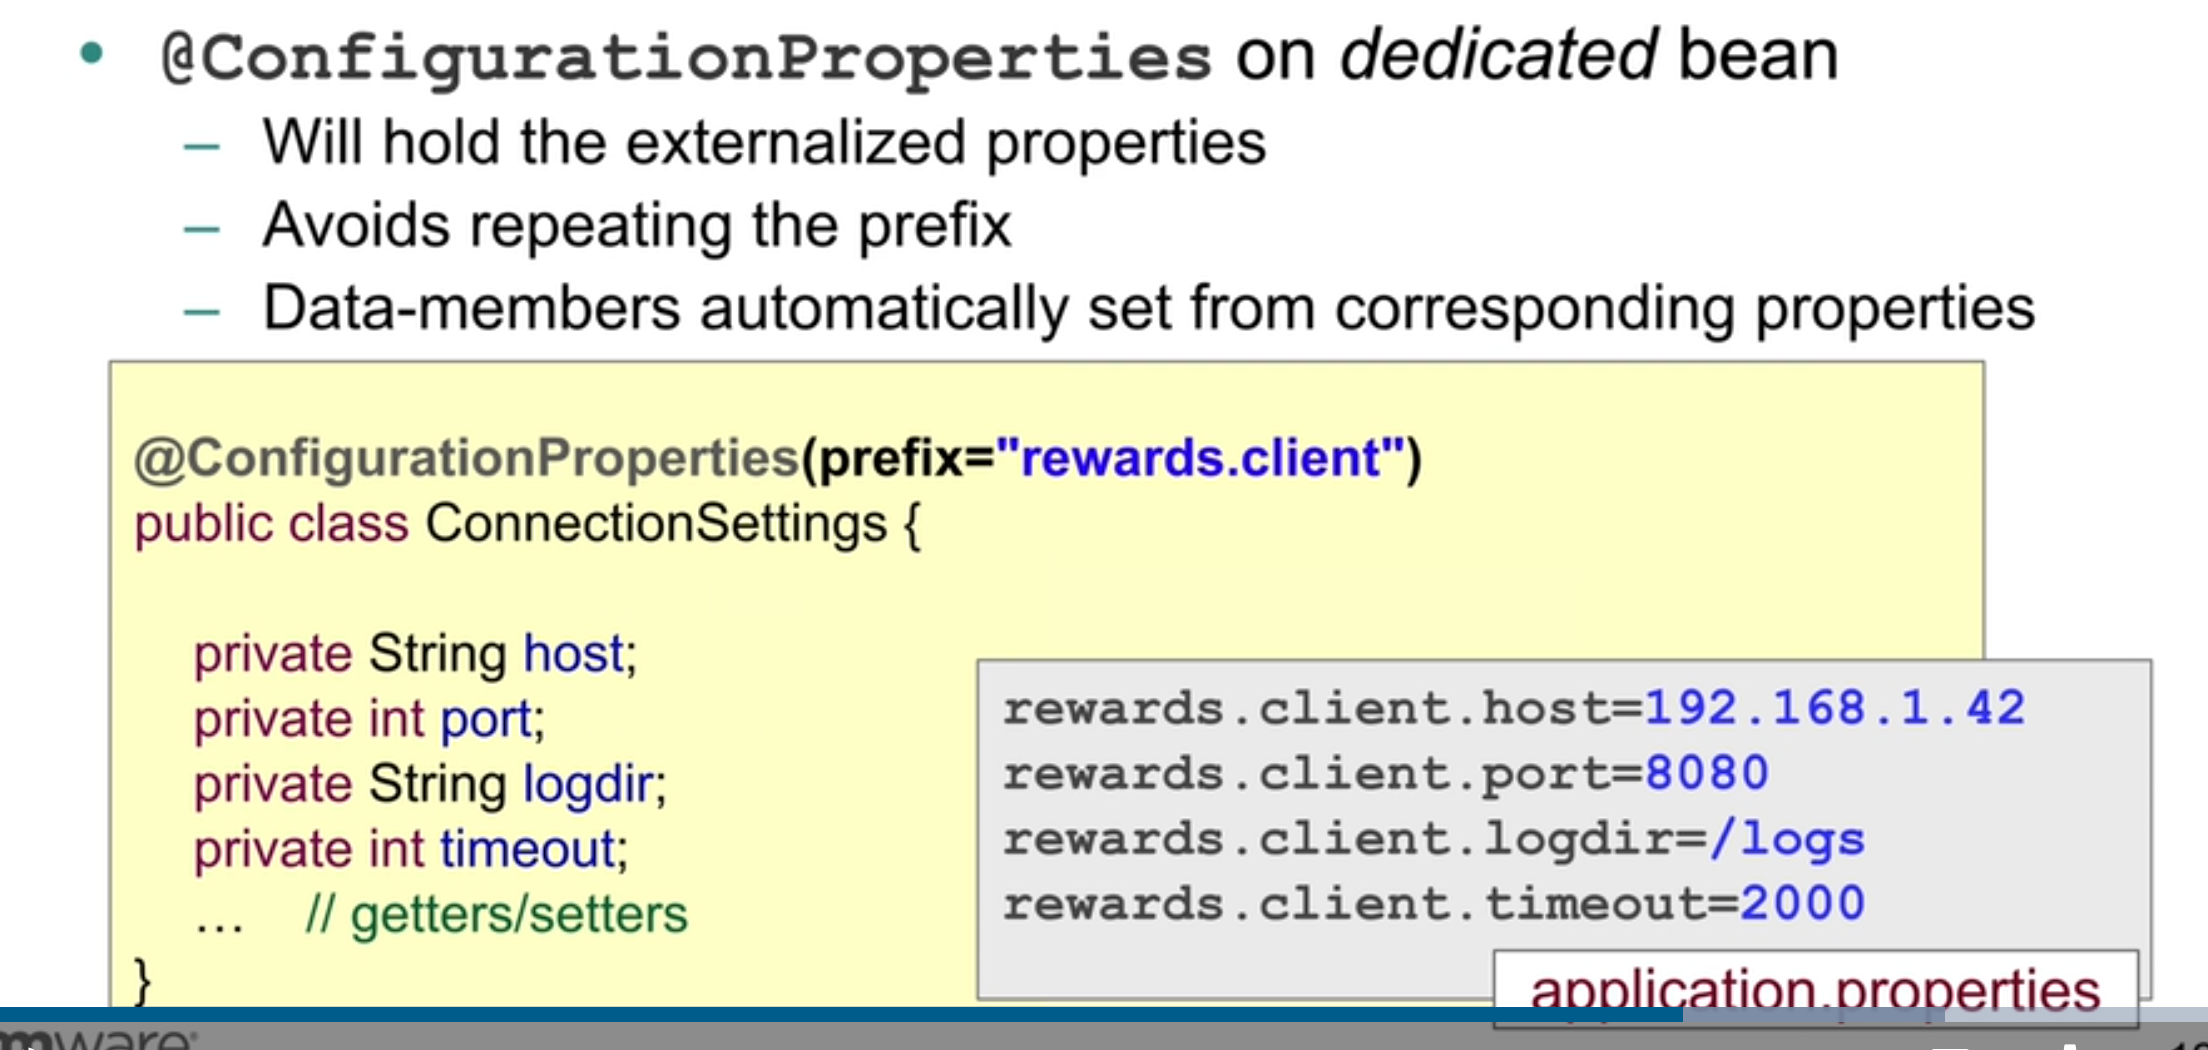
\includegraphics[width=1\linewidth]{configurationproperties}
    \caption{}
    \label{fig:configurationproperties}
\end{figure}

\subsubsection{@ConditionalOnX}

Determine what auto configuration does. For example: @ConditionalOnBean, @ConditionalOnMissingBean, @ConditionalOnClass, @ConditionalOnMissingClass, @ConditionalOnProperty.

For example, @Profile is such a condition.

\subsubsection{RestController}

Includes @Controller and @ResponseBody.

\begin{figure}
    \centering
    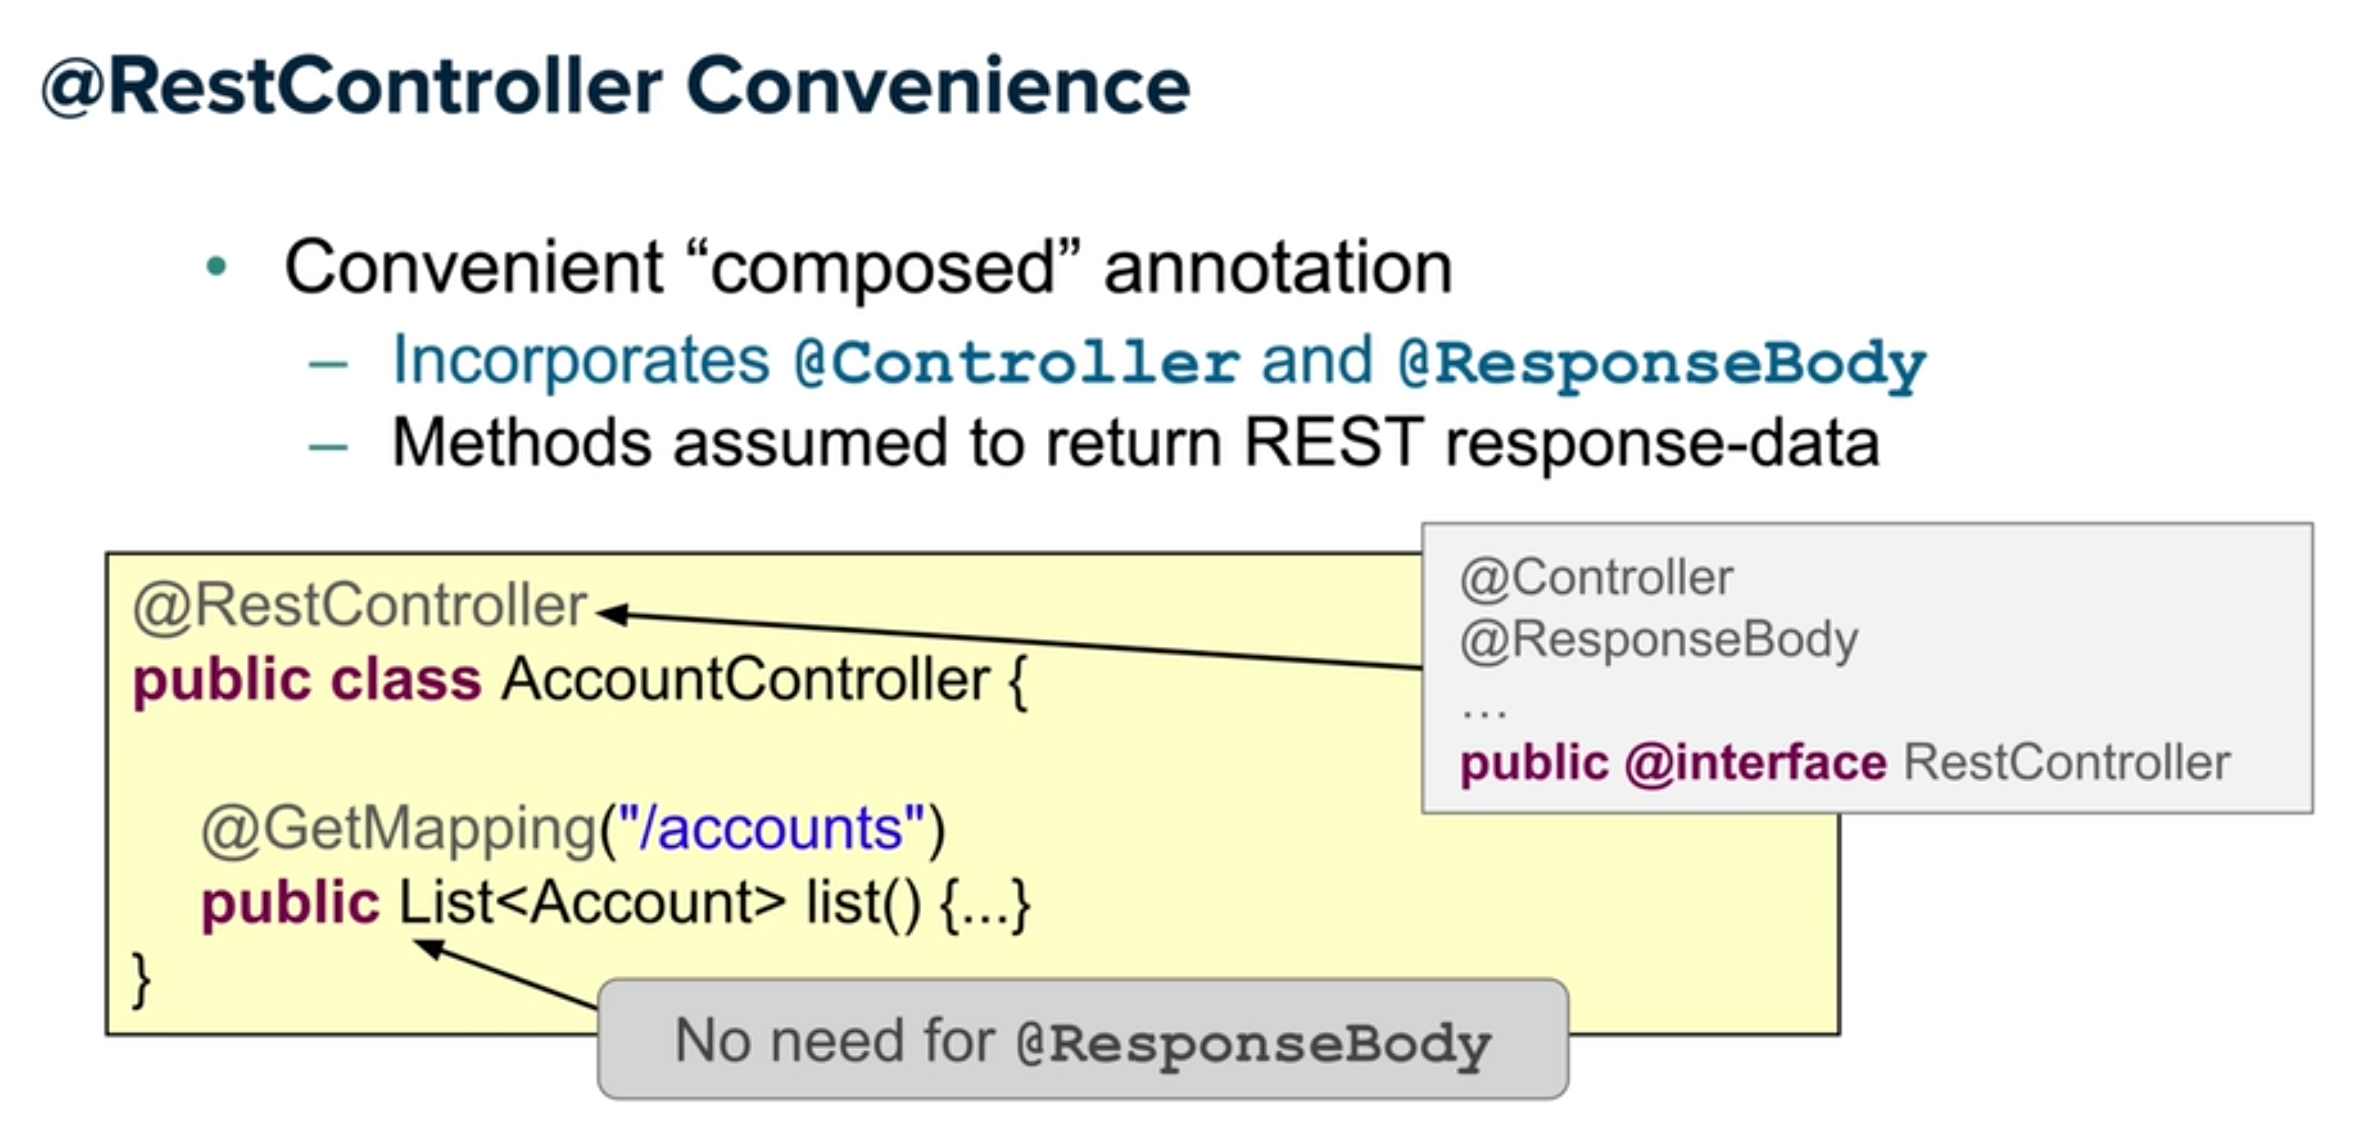
\includegraphics[width=1\linewidth]{restcontroller}
    \caption{RestController convenience annotation.}
    \label{fig:restcontroller}
\end{figure}

\subsubsection{Request URI Decomposition: @RequestParam, @PathVariable}

Do implicit type conversion of arguments.

\begin{lstlisting}
    // localhost:8080/account?userid=12345
    @GetMapping("/account")
    public List<Account> list(@RequestParam("userid"} int userid) {}

    // localhost:8080/accounts/12345
    @GetMapping("/accounts/{accountId}")
    public Account find (@PathVariable("accountId"} long id) {}

    // if argument name is missing, will take from the mapping
    // could also have

    // localhost:8080/account?overdrawn=12345
    @GetMapping("/account")
    public List<Account> list(@RequestParam int overdrawn) {}

    // localhost:8080/accounts/12345
    @GetMapping("/accounts/{accountId}")
    public Account find (@PathVariable long id) {}

    // localhost:8080/accounts/12345?overdrawn=true
    @GetMapping("/accounts/{accountId}")
    public Account find (
        @PathVariable long accountId,
        @RequestParam boolean overdrawn
    ) {}



\end{lstlisting}

\subsubsection{@ResponseBody}

Causes Java objects returned by the Controller to be processed by HttpMessageConverters in order to return information to the client in the form requested in the Accept header.

\subsubsection{@ResponseStatus}

    Used to return a status other than 200.

    \begin{lstlisting}
        @ResponseStatus(HttpStatus.NO_CONTENT)
        public void updateOrder(...){}
    \end{lstlisting}

\subsubsection{@RequestBody}

    Used to extract the request body.

\section{Aware Interfaces}

    Indicates that the bean is eligible to be notified by the Spring container through the callback methods.
    A typical use case for BeanNameAware could be acquiring the bean name for logging or wiring purposes. For the BeanFactoryAware it could be the ability to use a spring bean from legacy code.
    In most cases, we should avoid using any of the Aware interfaces, unless we need them. Implementing these interfaces will couple the code to the Spring framework.

\subsection{BeanNameAware}

    Makes the object aware of the bean name defined in the container.

\begin{lstlisting}
    public class MyBeanName implements BeanNameAware {
        @Override
        public void setBeanName(String beanName) {
            System.out.println(beanName);
        }
    }
    @Configuration
    public class Config {
        @Bean(name = "myCustomBeanName")
        public MyBeanName getMyBeanName() {
            return new MyBeanName();
        }
    }
    AnnotationConfigApplicationContext context
    = new AnnotationConfigApplicationContext(Config.class);
    MyBeanName myBeanName = context.getBean(MyBeanName.class);

\end{lstlisting}

\subsection{BeanFactoryAware}

    Provides access to the BeanFactory which created the object.

    \begin{lstlisting}
        public class MyBeanFactory implements BeanFactoryAware {
            private BeanFactory beanFactory;
            @Override
            public void setBeanFactory(BeanFactory beanFactory) throws BeansException {
                this.beanFactory = beanFactory;
            }
            public void getMyBeanName() {
                MyBeanName myBeanName = beanFactory.getBean(MyBeanName.class);
                System.out.println(beanFactory.isSingleton("myCustomBeanName"));
            }
        }
        MyBeanFactory myBeanFactory = context.getBean(MyBeanFactory.class);
        myBeanFactory.getMyBeanName();}
    \end{lstlisting}

\subsection{ApplicationContextAware}
    \begin{lstlisting}
        public class ApplicationContextAwareImpl implements ApplicationContextAware {
            @Override
            public void setApplicationContext(ApplicationContext applicationContext) throws BeansException {
                User user = (User) applicationContext.getBean("user");
                System.out.println("User Id: " + user.getUserId() + " User Name :" + user.getName());}}
    \end{lstlisting}


\section{Bean Naming}
\label{sec:bean-naming}
\subsection{Default Bean Naming}
\subsubsection{Class-level ("Annotation-based configuration")}
For an annotation used at the class level (@Component, @Service, @Controller), Spring uses the class name and converts the first letter to lowercase.
Custom names may be configured in the annotation's value attribute.

The type is determined from the annotated class, typically resulting in the actual
implementation class.

    \begin{lstlisting}
        @Service
        public class LoggingService { // bean name = loggingService

        }
    \end{lstlisting}

\subsubsection{Method-level ("Java configuration")}
When in a @Configuration class we use the @Bean annotation on a method, Spring uses the method name for the bean name.

    \begin{lstlisting}
        @Configuration
        public class AuditConfiguration {
            @Bean
            public AuditService audit() {
                return new AuditService();
            }
        }
    \end{lstlisting}

\subsection{Custom naming}

    \begin{lstlisting}
        @Component("myBean")
        public class MyCustomComponent {
        }
    \end{lstlisting}

   Custom names may be configured in @Bean's value attribute.

   The type is determined from the method return type, typically resulting in an interface.

\subsection{Naming Beans With @Bean and @Qualifier}
\subsubsection{@Bean With Value}
    The @Bean annotation is applied at the method level, and by default, Spring uses the method name as a bean name. We can override this using the @Bean annotation.

     \begin{lstlisting}
        @Configuration
        public class MyConfiguration {
            @Bean("beanComponent")
            public MyCustomComponent myComponent() {
                return new MyCustomComponent();
            }
        }
    \end{lstlisting}

\subsubsection{@Qualifier With Value}
    We can also use the @Qualifier annotation to name the bean.

    \begin{lstlisting}
        @Component
        @Qualifier("cat")
        public class Cat implements Animal {
            @Override
            public String name() {
                return "Cat";
            }
        }
        @Component
        @Qualifier("dog")
        public class Dog implements Animal {
            @Override
            public String name() {
                return "Dog";
            }
        }
        @Service
        public class PetShow {
            private final Animal dog;
            private final Animal cat;

            public PetShow (@Qualifier("dog")Animal dog, @Qualifier("cat")Animal cat) {
                this.dog = dog;
                this.cat = cat;
            }
            public Animal getDog() {
                return dog;
            }
            public Animal getCat() {
                return cat;
            }
        }
        \end{lstlisting}

\section{Spring Expression Language vs. Property Evaluation}

    Expressions in @Value annotations are of two types:

    \begin{itemize}
        \item Expressions starting with \$. Such expressions reference a property name in the application’s environment. These expressions are evaluated by the PropertySourcesPlaceholderConfigurer BeanFactoryPostProcessor prior to bean creation and can only be used in @Value annnotations.
        \item Expressions starting with \#.
        These expressions are parsed by a SpEL expression parser, and are evaluated by a SpEL expression instance.
    \end{itemize}

    In some cases, both can be used. For example, property values by default are Strings, but may be converted to primitives implicitly. So, both of these work:

    \begin{lstlisting}
        @Value("${daily.limit}")
        int limit;

        @Value("#{environment['daily.limit']}")
        int limit;
    \end{lstlisting}

    But if computations are to be performed, or object types are required, SpEL has to be used:

    \begin{lstlisting}
        // NO
        @Value("${daily.limit} * 2")

        // instead, do
        @Value("#{new Integer(environment['daily.limit']}) * 2")
    \end{lstlisting}

    To provide defaults, use a colon with property evaluation, and ?: in SpEL.

    \begin{lstlisting}
        @Value("${daily.limit}: 1000")
        int limit;

        @Value("#{environment['daily.limit']} ?: 1000")
        int limit;
    \end{lstlisting}

    In addition to application-defined beans, SpEL can make use of beans implicitly provided by Spring, namely environment, systemProperties, and systemEnvironment.

\section{AOP in Spring}

\subsection{Core AOP concepts}

\subsubsection{Join Point}

A point during the execution of a program, such as the execution of a method or the handling of an exception.

In Spring AOP, a join point always represents a method execution.


\subsubsection{Point Cut}

An expression that selects one or more join points.

Although Spring supports various AspectJ pointcut designators, the most commonly used one is \lstinline{execution}.

For this designator, the syntax pattern is as follows:

\begin{lstlisting}
    execution(
    modifiers-pattern?
    ret-type-pattern
    declaring-type-pattern.?name-pattern(param-pattern)
    throws-pattern?
    )
\end{lstlisting}

All parts except the returning type pattern (ret-type-pattern in the preceding snippet), the name pattern, and the parameters pattern are optional.

\begin{itemize}
    \item The returning type pattern determines what the return type of the method must be in order for a join point to be matched. * is most frequently used as the returning type pattern. It matches any return type. A fully-qualified type name matches only when the method returns the given type.
    \item  The name pattern matches the method name. You can use the * wildcard as all or part of a name pattern. If you specify a declaring type pattern, include a trailing . to join it to the name pattern component.
    \item The parameters pattern is slightly more complex: () matches a method that takes no parameters, whereas (..) matches any number (zero or more) of parameters. The (*) pattern matches a method that takes one parameter of any type. (*,String) matches a method that takes two parameters. The first can be of any type, while the second must be a String.

\end{itemize}

Examples:

\begin{lstlisting}
// The execution of any public method:
execution(public * *(..))

// The execution of any method with a name that begins with set:
execution(* set*(..))

// The execution of any method defined by the AccountService interface:
execution(* com.xyz.service.AccountService.*(..))

// The execution of any method defined in the service package:
execution(* com.xyz.service.*.*(..))

//The execution of any method defined in the service package or one of its sub-packages:
execution(* com.xyz.service..*.*(..))

// There is one directory between rewards and restaurant.
execution(* rewards.*.restaurant.*.*(..))

// There are 0 or more directories between rewards and restaurant.
execution(* rewards..restaurant.*.*(..))

// There must be at least 1 directory before restaurant.
// omitting the star is not allowed
execution(* *..restaurant.*.*(..))

// Any join point (method execution only in Spring AOP) within the service package:
within(com.xyz.service.*)

// Any join point (method execution only in Spring AOP) within the service package or one of its sub-packages:
within(com.xyz.service..*)

// Any join point (method execution only in Spring AOP) where the proxy implements the AccountService interface:
this(com.xyz.service.AccountService)

// Any join point (method execution only in Spring AOP) where the target object implements the AccountService interface:
target(com.xyz.service.AccountService)

// Any join point (method execution only in Spring AOP) that takes a single parameter and where the argument passed at runtime is Serializable:
args(java.io.Serializable)

// Note that the pointcut given in this example is different from execution(* *(java.io.Serializable)). The args version matches if the argument passed at runtime is Serializable, and the execution version matches if the method signature declares a single parameter of type Serializable.

// Any join point (method execution only in Spring AOP) where the target object has a @Transactional annotation:
@target(org.springframework.transaction.annotation.Transactional)

// Any join point (method execution only in Spring AOP) where the declared type of the target object has an @Transactional annotation:
@within(org.springframework.transaction.annotation.Transactional)

// Any join point (method execution only in Spring AOP) where the executing method has an @Transactional annotation:
@annotation(org.springframework.transaction.annotation.Transactional)

// Any join point (method execution only in Spring AOP) which takes a single parameter, and where the runtime type of the argument passed has the @Classified annotation:
@args(com.xyz.security.Classified)

// Any join point (method execution only in Spring AOP) on a Spring bean named tradeService:
bean(tradeService)

// Any join point (method execution only in Spring AOP) on Spring beans having names that match the wildcard expression *Service:
bean(*Service)
\end{lstlisting}

\subsubsection{Advice}


Code to be executed at a particular join point.
Types:

\begin{itemize}
    \item Before-advice is executed before calling the target method.
    \begin{lstlisting}
        @Before("execution(void set*(*))    \end{lstlisting}
    \item
    After-advice is executed after the target method, whatever its outcome.
    \begin{lstlisting}
        @Before("execution(void set*(*))
    \end{lstlisting}
    \item
    After-returning: executed after the target returns successfully. This advice will never execute if the target throws any exception.
    The return parameter also gives access to the returned object.
    \begin{lstlisting}
        @AfterReturning(value="execution(* service..*(..))", return="reward")
        public void audit(Join Point jp, Reward reward) {
            auditService.logEvent(jp.getSignature() + ": " + reward.toString());
        }
    \end{lstlisting}
    \item
    After-throwing: executed after the target throws an exception.
    Also gives access to the exception.
    \begin{lstlisting}
        // Repositories in any package
        @AfterThrowing(value="execution(* *..Repository.*(..))", throwing="e")
        // also have to match the type of the exception
        public void report(JoinPoint jp, DataAccessException e) {
        mailService.mailFailure(jp.getSignature(), e);
        }
    \end{lstlisting}
    While this advice cannot prevent an exception to be thrown, it can throw a more user-friendly exception instead:
    \begin{lstlisting}
        @AfterThrowing(value="execution(* *..Repository.*(..))", throwing"e")
        public void report(JoinPoint jp, DataAccessException e) {
            mailService.mailFailure(jp.getSignature(), e);
            throw new RewardsException();
        }
    \end{lstlisting}
    \item
    Around: executed two times, before and after invocation of the target method. Must call proceed() to delegate to the target. See \ref{fig:around-advice}.
    \begin{figure}
        \centering
        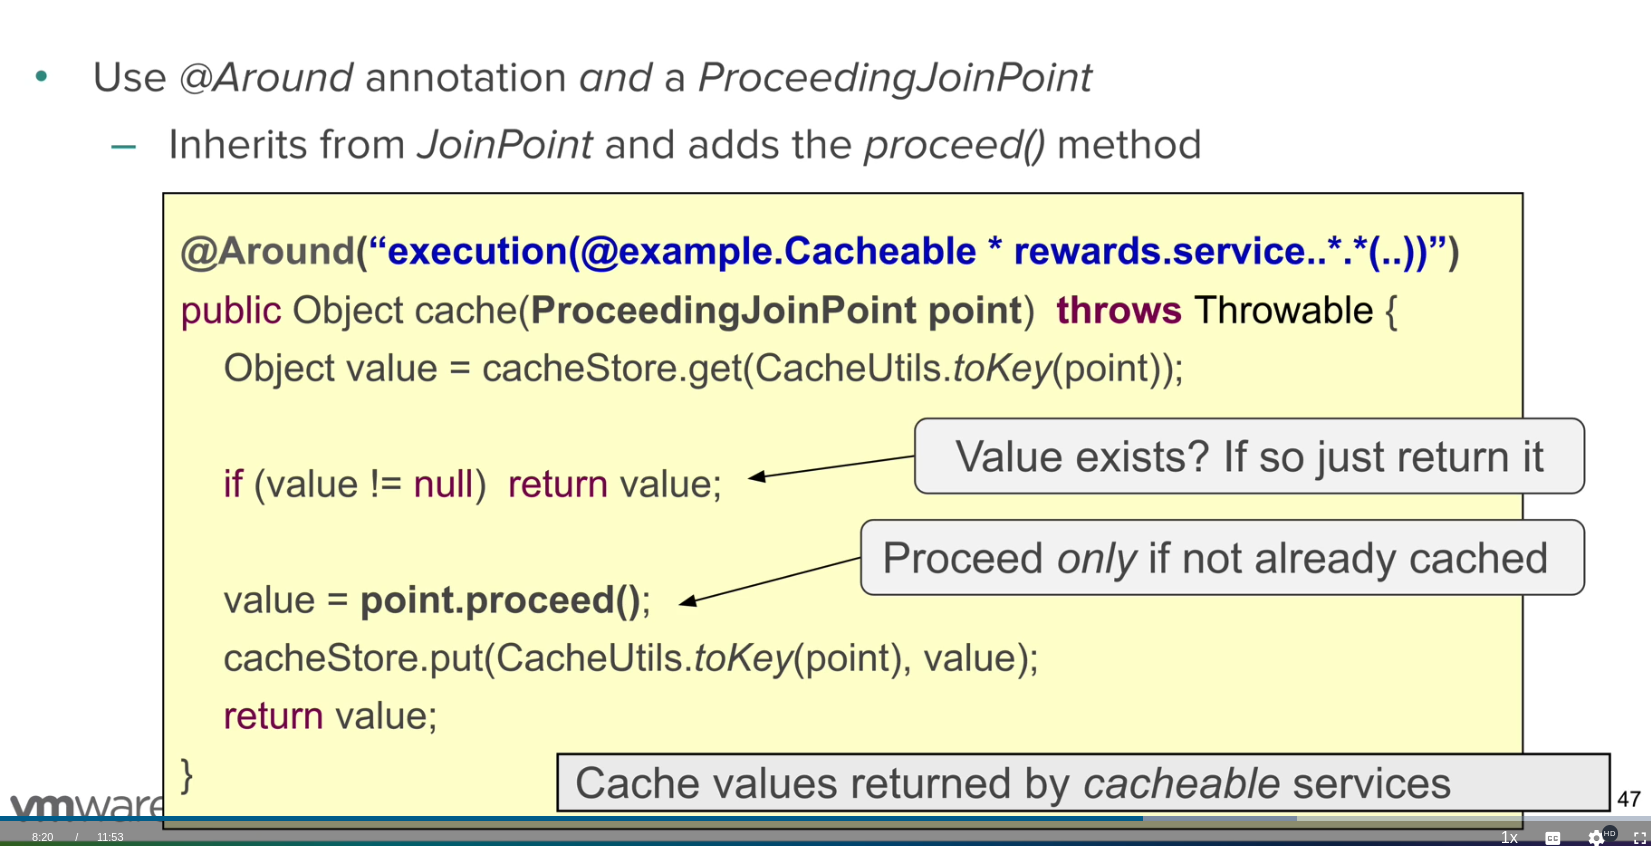
\includegraphics[width=1\linewidth]{around-advice}
        \caption{Around Advice}
        \label{fig:around-advice}
    \end{figure}

\end{itemize}

\subsubsection{Aspect}

The combination of point cut and advice. The @aspect annotation needs to be explicitly enabled by @EnableAspectJConfiguration set in the context (Config) class.

This will cause an extension of AbstractAutoProxyCreator to run, a BeanPostProcessor that wraps a bean with an AOP proxy. See \ref{fig:autoproxycreator}.

\begin{figure}
    \centering
    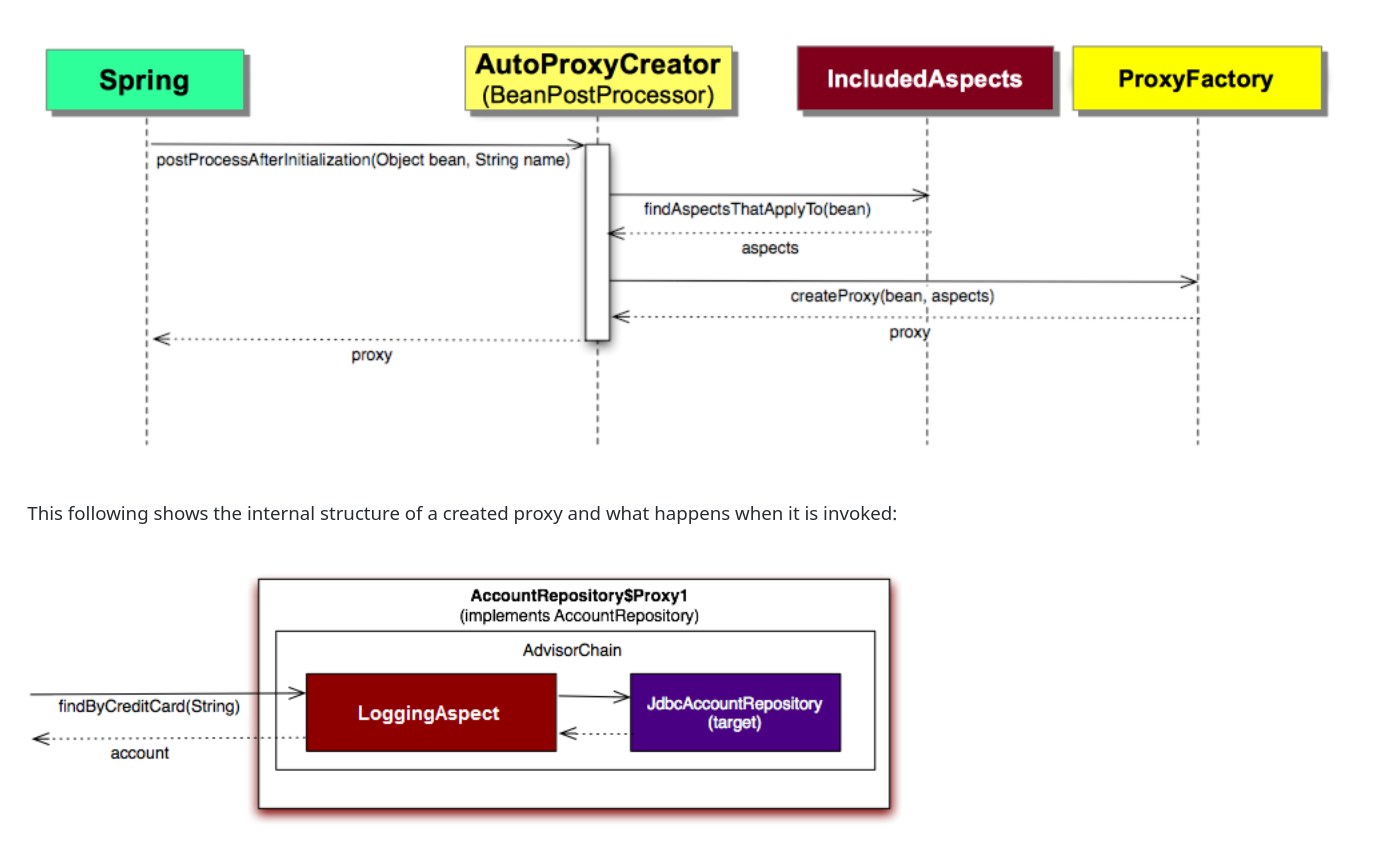
\includegraphics[width=1\linewidth]{autoproxycreator}
    \caption{Proxy Creation.}
    \label{fig:autoproxycreator}
\end{figure}

An aspect can get context information by injecting the JoinPoint into the advice. See fig. \ref{fig:AOP-join-point}.

\begin{figure}
    \centering
    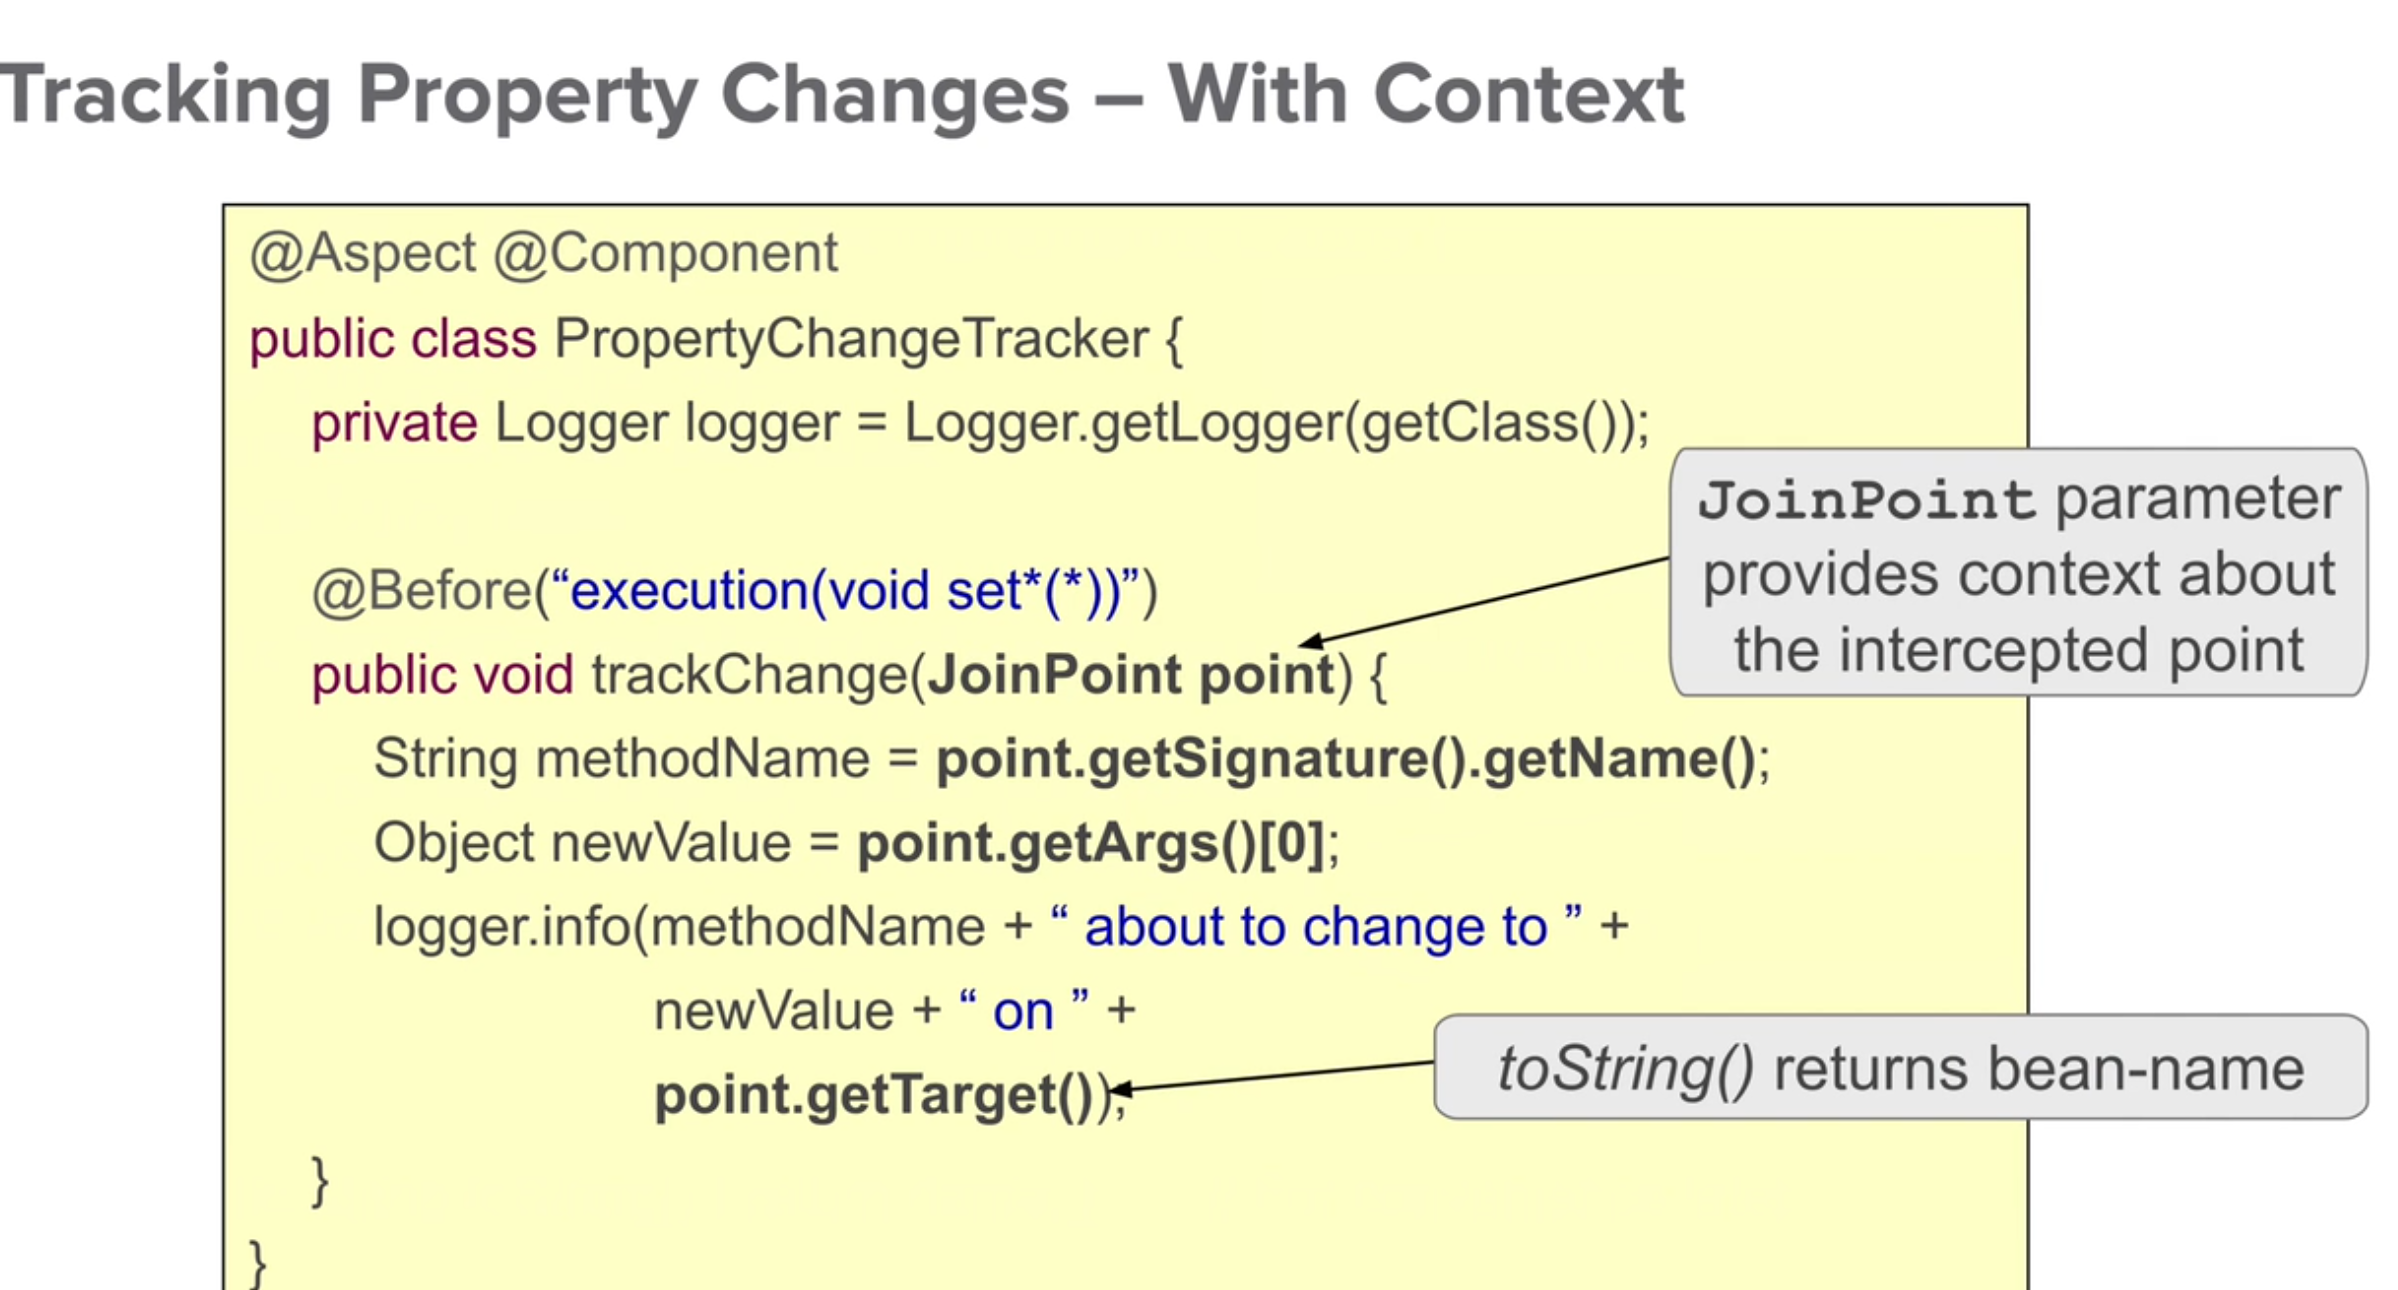
\includegraphics[width=1\linewidth]{AOP-join-point}
    \caption{Automatic JoinPoint injection}
    \label{fig:AOP-join-point}
\end{figure}

\begin{lstlisting}
    public abstract class AbstractAutoProxyCreator extends ProxyProcessorSupport
    implements SmartInstantiationAwareBeanPostProcessor, BeanFactoryAware {
        //...

        @Override
        public Object postProcessBeforeInstantiation(Class<?> beanClass, String beanName) {
            Object cacheKey = getCacheKey(beanClass, beanName);

            if (!StringUtils.hasLength(beanName) || !this.targetSourcedBeans.contains(beanName)) {
                if (this.advisedBeans.containsKey(cacheKey)) {
                    return null;
                }
                if (isInfrastructureClass(beanClass) || shouldSkip(beanClass, beanName)) {
                    this.advisedBeans.put(cacheKey, Boolean.FALSE);
                    return null;
                }
            }
        }

        @Override
        public Object postProcessAfterInitialization(@Nullable Object bean, String beanName) {
            if (bean != null) {
                Object cacheKey = getCacheKey(bean.getClass(), beanName);
                if (this.earlyProxyReferences.remove(cacheKey) != bean) {
                    return wrapIfNecessary(bean, beanName, cacheKey);
                }
            }
            return bean;
        }
    }
\end{lstlisting}

\section{JPA}
\subsection{Repository Query Language}

Example (see \url{  https://docs.spring.io/spring-data/commons/reference/repositories/query-methods-details.html}):


\begin{lstlisting}
   interface PersonRepository extends Repository<Person, Long> {

       List<Person> findByEmailAddressAndLastname(EmailAddress emailAddress, String lastname);

       // Enables the distinct flag for the query
       List<Person> findDistinctPeopleByLastnameOrFirstname(String lastname, String firstname);
       List<Person> findPeopleDistinctByLastnameOrFirstname(String lastname, String firstname);

       // Enabling ignoring case for an individual property
       List<Person> findByLastnameIgnoreCase(String lastname);
       // Enabling ignoring case for all suitable properties
       List<Person> findByLastnameAndFirstnameAllIgnoreCase(String lastname, String firstname);

       // Enabling static ORDER BY for a query
       List<Person> findByLastnameOrderByFirstnameAsc(String lastname);
       List<Person> findByLastnameOrderByFirstnameDesc(String lastname);
   }
\end{lstlisting}

\subsection{Reserved Method Names}

    Reserved methods like CrudRepository.findById (or just findById) are targeting the identifier property regardless of the actual property name used in the declared method.
    Example:

\begin{lstlisting}
    class User {
        //The identifier property (primary key).
        @Id Long pk;

        // A property named id, but not the identifier.
        Long id;
    }

    interface UserRepository extends Repository<User, Long> {

        // Targets the pk property (the one marked with @Id which is considered to be the identifier) as it refers to a CrudRepository base repository method.
        Optional<User> findById(Long id);

        // Targets the pk property by name as it is a derived query.
        Optional<User> findByPk(Long pk);

        // Targets the id property by using the descriptive token between find and by to avoid collisions with reserved methods.
        Optional<User> findUserById(Long id);
    }

\end{lstlisting}

\section{Paging, Iterating Large Results, Sorting and Limiting}

    Spring recognizes certain specific types like Pageable, Sort and Limit, to apply pagination, sorting and limiting to your queries dynamically.
    Example:

\begin{lstlisting}
    Page<User> findByLastname(String lastname, Pageable pageable);

    Slice<User> findByLastname(String lastname, Pageable pageable);

    List<User> findByLastname(String lastname, Sort sort);

    List<User> findByLastname(String lastname, Sort sort, Limit limit);

    List<User> findByLastname(String lastname, Pageable pageable);
\end{lstlisting}

\section{Repository Query Keywords}

\begin{lstlisting}
    // General query method returning typically the repository type, a Collection or Streamable subtype or a result wrapper such as Page, GeoResults or any other store-specific result wrapper. Can be used as findBy..., findMyDomainTypeBy... or in combination with additional keywords.
    find...By, read...By, get...By, query...By, search...By, stream...By

    // Exists projection, returning typically a boolean result.
    exists...By

    // Count projection returning a numeric result.
    count...By

    //  Delete query method returning either no result (void) or the delete count.
    delete...By, remove...By

    //  Limit the query results to the first <number> of results. This keyword can occur in any place of the subject between find (and the other keywords) and by.
    ...First<number>..., ...Top<number>...

    //  Use a distinct query to return only unique results. Consult the store-specific documentation whether that feature is supported. This keyword can occur in any place of the subject between find (and the other keywords) and by.
    ...Distinct...
\end{lstlisting}

\section{Supported query method predicate keywords and modifiers}

\begin{table}[ht]
\begin{tabular}{ | r | r |}
    \hline
    Logical keyword &	Keyword expressions \\
    \hline
    AND & And \\
    OR &  Or \\
    AFTER & After, IsAfter \\
    BEFORE & Before, IsBefore\\
    CONTAINING&Containing, IsContaining, Contains\\
    BETWEEN&Between, IsBetween\\
    ENDING\_WITH&EndingWith, IsEndingWith, EndsWith\\
    EXISTS&Exists\\
    FALSE&False, IsFalse\\
    GREATER\_THAN&GreaterThan, IsGreaterThan\\
    GREATER\_THAN\_EQUALS&GreaterThanEqual, IsGreaterThanEqual\\
    IN&In, IsIn\\
    IS&Is, Equals, (or no keyword)\\
    IS\_EMPTY&IsEmpty, Empty\\
    IS\_NOT\_EMPTY&IsNotEmpty, NotEmpty\\
    IS\_NOT\_NULL&NotNull, IsNotNull\\
    IS\_NULL&Null, IsNull\\
    LESS\_THAN&LessThan, IsLessThan\\
    LESS\_THAN\_EQUAL&LessThanEqual, IsLessThanEqual\\
    LIKE&Like, IsLike\\
    NEAR&Near, IsNear\\
    NOT&Not, IsNotNOT\_INNotIn, IsNotIn\\
    NOT\_LIKE&NotLike, IsNotLike\\
    REGEX&Regex, MatchesRegex, Matches\\
    STARTING\_WITH&StartingWith, IsStartingWith, StartsWith\\
    TRUE&True, IsTrue\\
    WITHIN&Within, IsWithin\\
    \hline
\end{tabular}
\end{table}

    In addition to filter predicates, the following list of modifiers is supported:
    \begin{itemize}
        \item IgnoreCase, IgnoringCase
        \item AllIgnoreCase, AllIgnoringCase
        \item OrderBy... (e. g. OrderByFirstnameAscLastnameDesc).
    \end{itemize}


\section{Supported query method predicate keywords and modifiers}

    \begin{table}[ht]
    \begin{tabular}{ | r | r |}
    \hline
    Logical keyword& 	Keyword expressions \\

    AND&


    And\\

    OR&


    Or\\

    AFTER&


    After, IsAfter\\

    BEFORE&


    Before, IsBefore\\

    CONTAINING&


    Containing, IsContaining, Contains\\

    BETWEEN&


    Between, IsBetween\\

    ENDING\_WITH&


    EndingWith, IsEndingWith, EndsWith\\

    EXISTS&


    Exists\\

    FALSE&


    False, IsFalse\\

    GREATER\_THAN&


    GreaterThan, IsGreaterThan\\

    GREATER\_THAN\_EQUALS&


    GreaterThanEqual, IsGreaterThanEqual\\

    IN&


    In, IsIn\\

    IS&


    Is, Equals, (or no keyword)\\

    IS\_EMPTY&


    IsEmpty, Empty\\

    IS\_NOT\_EMPTY&


    IsNotEmpty, NotEmpty\\

    IS\_NOT\_NULL&


    NotNull, IsNotNull\\

    IS\_NULL&


    Null, IsNull\\

    LESS\_THAN&


    LessThan, IsLessThan\\

    LESS\_THAN\_EQUAL&


    LessThanEqual, IsLessThanEqual\\

    LIKE&


    Like, IsLike\\

    NEAR&


    Near, IsNear\\

    NOT&


    Not, IsNot\\

    NOT\_IN&


    NotIn, IsNotIn\\

    NOT\_LIKE&


    NotLike, IsNotLike\\

    REGEX&


    Regex, MatchesRegex, Matches\\

    STARTING\_WITH&


    StartingWith, IsStartingWith, StartsWith\\

    TRUE&


    True, IsTrue\\

    WITH&


    Within, IsWithin\\
    \hline
    \end{tabular}
\end{table}

\section{Spring Boot Web}

Architecture Overview:

\begin{figure}
    \centering
    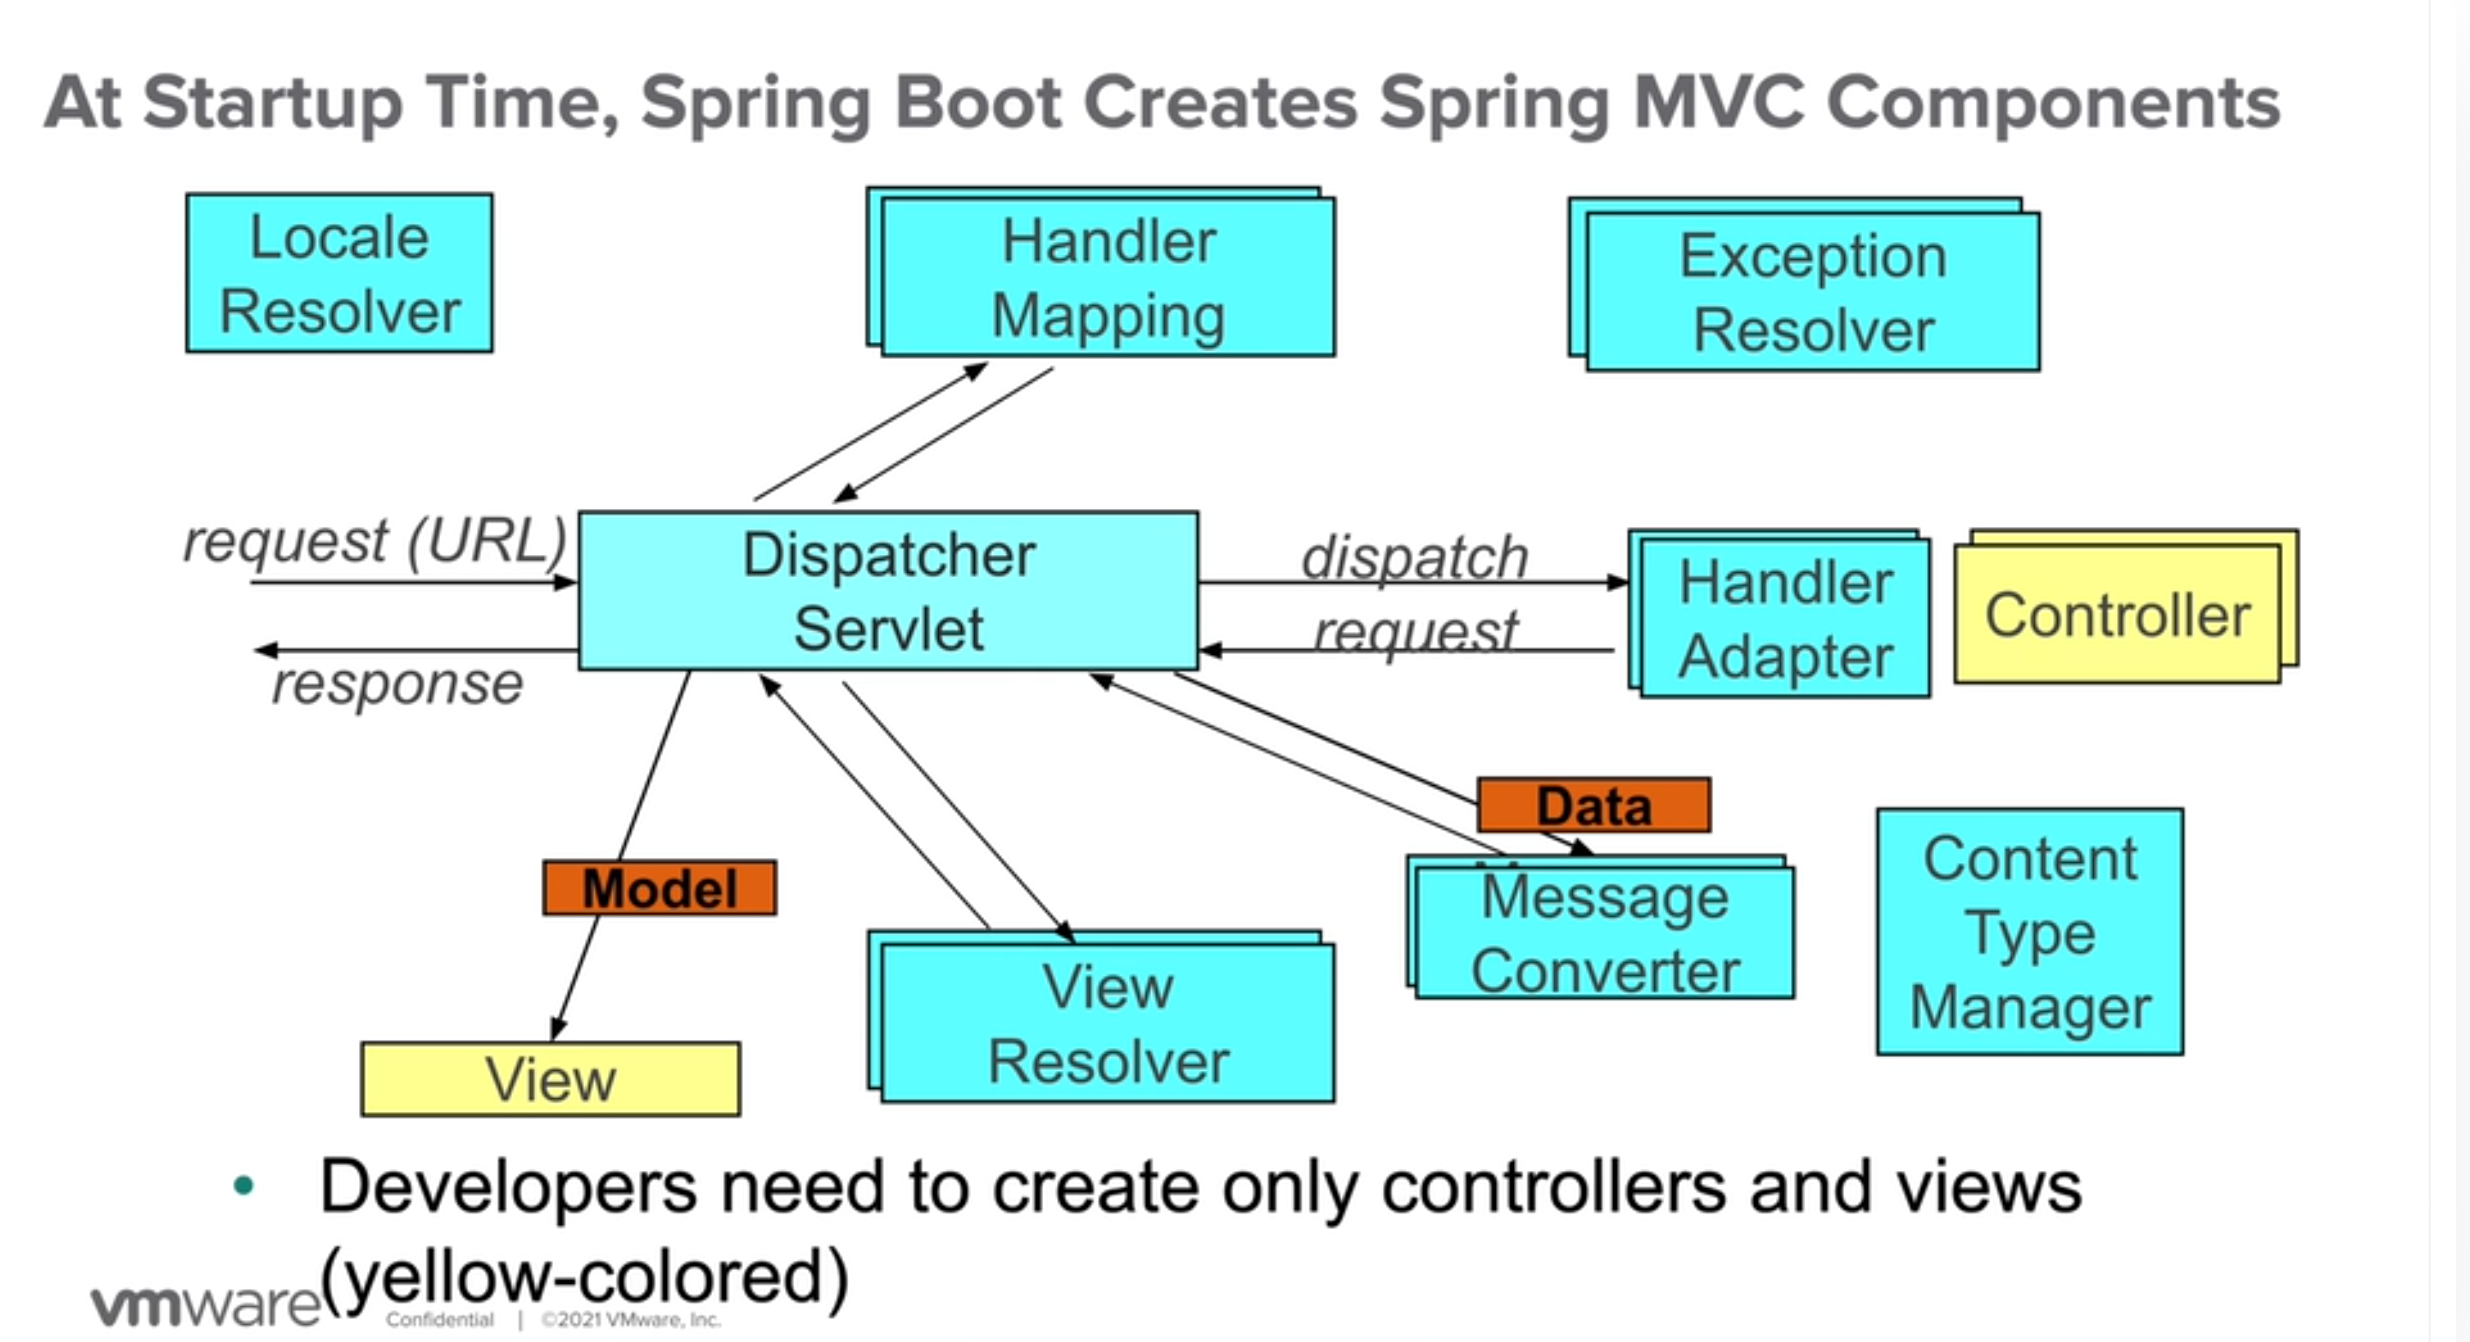
\includegraphics[width=1\linewidth]{spring-web}
    \caption{Spring Boot Web Architecture Overview}
    \label{fig:spring-web}
\end{figure}


\begin{lstlisting}

\end{lstlisting}

\begin{lstlisting}

\end{lstlisting}

\begin{lstlisting}

\end{lstlisting}

\begin{lstlisting}

\end{lstlisting}

\begin{lstlisting}

\end{lstlisting}

\begin{lstlisting}

\end{lstlisting}

\begin{lstlisting}

\end{lstlisting}






\end{document}




























